\chapter{What is Docker?}
Docker is an open-source platform for developing, deploying and running applications. Docker allows to separate applications from infrastructure using environment virtualization, which is empowered by virtualization support  in kernel and by tools that help to manage and deploy applications. Containers are used again, but they are not as independent as OpenVZ containers for example. Docker uses containerization support in kernel, so applications share kernel with the host machine. This makes containers more lightweight, faster to run and portable. Docker allows more advantages thanks to it is wrapping basic kernel virtualization

\section{Docker architecture}
Docker daemon runs on the host machine and manages all Docker images and containers. Docker client communicates with this daemon to create images and to upload them on Docker registry. The figure \ref{fig:docker-architecture} shows the whole concept of it.

\subsection{Docker image}
Docker image is a read-only template. It contains a chosen operating system and a set of installed applications. Images used to run simple binary program can also start from scratch.

\subsection{Docker container}
Docker container is a structure holding everything what application may need to run. Each container is based on an image. There can be multiple containers based on the same image, all of them can be started, stopped, moved or deleted individually and users can attach to any of them. Containers provide an isolated and a secure platform for applications.

\subsection{Docker registry}
Docker registry is a server-side application holding images. It is a storage, where clients can push their images so anyone can pull them and run containers based on them.

\begin{figure}[htb]\centering
  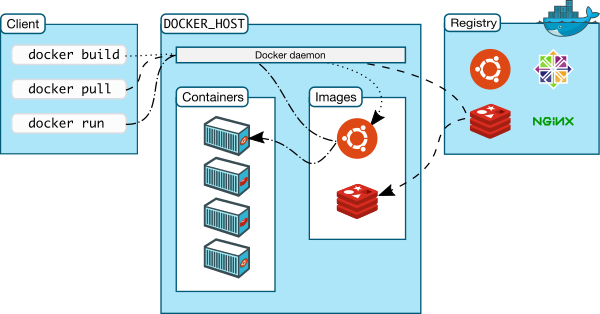
\includegraphics[width=1\textwidth]{images/dockerarchitecture.png}
  \caption
    [Docker architecture]
    {Docker architecture \cite{dockerdocs}}
  \label{fig:docker-architecture}
\end{figure}